\chapter{Implementation}\label{implementation}

The most promising vector tile specification was proposed by Mapbox.
%\marginpar{The Mapbox Vector Tile Specification is compared with other vector tile formats in chapter \ref{vector-tile-formats}}
They provide many open source tools to manage vector tiles. Instead of implementing existing tools and approaches as many existing tools
as possible were used to speed up development.
Because of this the implementation consists mostly of docker containers which do a specific task.

\section{Mapping}

Imposm 3 requires a custom mapping file to decide which tags and geometries are mapped into which table.

The example data mapping\cite{81_imposm.org_2015} defines that geometries of type polygon with the key value pairs \texttt{natural=wood}, \texttt{natural=land} and \texttt{tourism=zoo} should be mappend into the \texttt{landusages} table.

\begin{yamlcode}
tables:
   landusages:
     type: polygon
     mapping:
       natural: [wood, land]
       tourism: [zoo]
\end{yamlcode}

Instead of mapping all values of a certain key a explicit mapping strategy has been chosen. Each tag was explicitly defined in the mapping. This required mapping a lot of tags (to map all sport POIs over 79 tags are mapped) but has the benefit of knowing exactly which tags are in the database which makes querying and filtering easier.

\begin{figure}[H]
\centering
  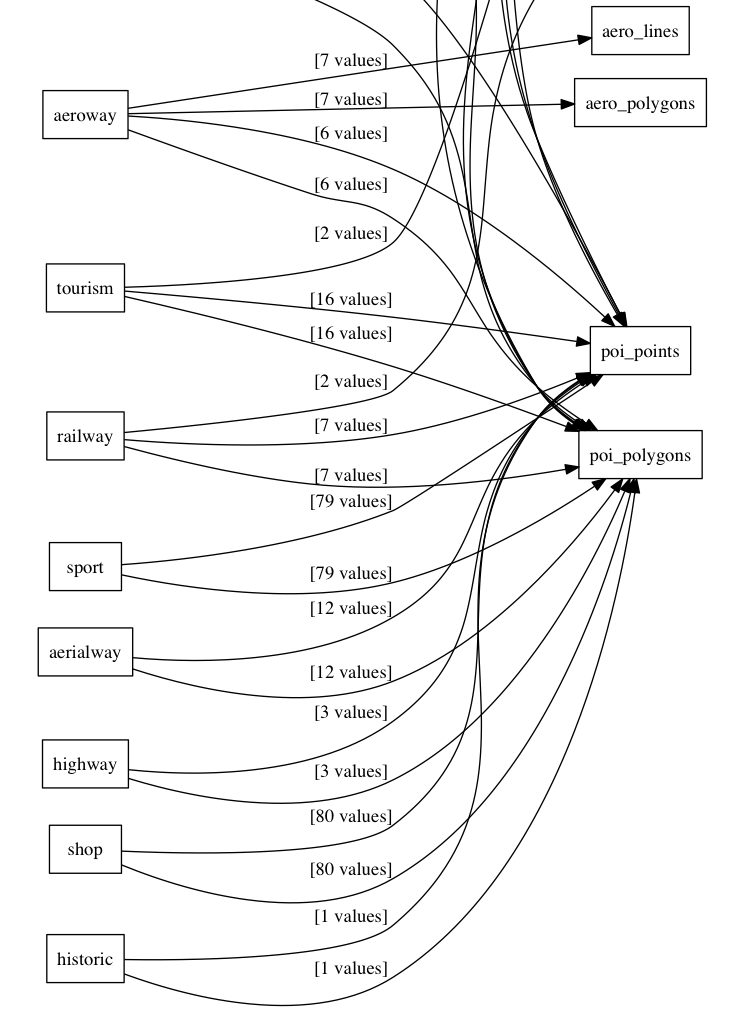
\includegraphics[width=1\textwidth]{images/mapping_keys.png}
  \caption{Mapping of tags to tables}
\end{figure}



\section{Database Schema}

This section describes the implementation details of the database schema.

\subsection{OSM id}
All tables and views that are derived from \osm{} data has the original id\cite{82_wiki.openstreetmap.org_2015}
to trace back the data and be able to query a distinct \osm{} feature in a visual style.

\subsection{Translations}
All features which are label layers will contain several translations.
The translations are directly mapped from the suffixed language code \cite{83_wiki.openstreetmap.org_2015}. If a field is not available in the language, the local name is used.

\begin{table}[H]
\centering
    \begin{tabular}{ll}
    \hline
     Field    & 	Description                                    \\
    \hline
    name      & Local name  \\
    name\_en	 & English                          \\
    name\_es	 & Spanish                          \\
    name\_fr	 & French                           \\
    name\_de	 & German                           \\
    name\_ru	 & Russian                          \\
    name\_zh	 & Chinese                          \\
    \end{tabular}
    \caption{Translations of name field}
\end{table}

\subsection{Type and Class}
The class can be explained as a feature class. It is a categorization of an OSM value.
The type is the OSM value of the feature.

\section{Classification}
\label{classification}

The OpenStreetMap tagging schema has developed into a complex taxonomy of real-world feature classes and objects. \cite[p. 15]{haklay2008openstreetmap}. Map designers don't want to design
for each distinct object specifically which is why Mapbox and others abstract distinct key value pairs into so called feature classes. Mapbox calls those feature class simply class. Mapping created key value pairs into categories, cannot be automated
and there is no standard. This is why this is done by hand.
\\
A map designer that wants to style agricultural areas does not care
what type of field it is.

\begin{table}[H]
\centering
    \begin{tabular}{llll}
    Key      & Value      & Class       & Type           \\
    \hline
    landuse  & farm       & agriculture & orchard        \\
    building & farm       & agriculture & farm           \\
    landuse  & farmland   & agriculture & farmland       \\
    landuse  & farmyard   & agriculture & farmyard       \\
    landuse  & allotments & agriculture & allotments     \\
    landuse  & vineyard   & agriculture & vineyard       \\
    landuse  & vineyard   & agriculture & plant\_nursery
    \end{tabular}
    \caption{Classification of landuse feature class}
\end{table}

\subsection{Classification Format}

The classicifcations are written in a YAML based format.
Where each key in \texttt{classifications} denotes the classification name. The elements within each classification (e.g. \texttt{driveway} or \texttt{main} are the class name and the values below the class name (e.g. \texttt{primary}, \texttt{primary\_link} the OSM values to match.
The OSM keys are not matched explicitly - only the values.

\begin{yamlcode}
classifications:
  road:
    highway:
    - motorway
    - motorway_link
    - driveway
    main:
    - primary
    - primary_link
    - trunk
    - trunk_link
    - secondary
    - secondary_link
    - tertiary
    - tertiary_link
\end{yamlcode}

\subsection{Code Generation}

The readable classification format is taken and immutable SQL functions are generated
from the YAML source. These functions can then be used in the layer queres.

The example above will result in the following function.

\begin{sqlcode}
CREATE OR REPLACE FUNCTION classify_road(type VARCHAR)
RETURNS VARCHAR AS $$
  BEGIN
    RETURN CASE
      WHEN type IN ('motorway','motorway_link','driveway') THEN 'highway'
      WHEN type IN ('primary','primary_link',
                    'trunk','trunk_link',
                    'secondary','secondary_link',
                    'tertiary','tertiary_link') THEN 'main'
    END;
  END;
$$ LANGUAGE plpgsql IMMUTABLE;
\end{sqlcode}

Classifications are then baked into vector tile attributes
of geometries.

\begin{sqlcode}
SELECT
  geometry,
  classify_road(type) AS class,
  type AS type
FROM osm_roads
\end{sqlcode}

\section{Relative Importance}
\label{localrank}

To reduce label density on lower zoom levels, but still contain all data in e.g. zoom level 14, the \texttt{localrank} attribute indiciates how
important a label is compared to the labels in its neighbourhood.

\subsection{Calculating Rank}

\subsubsection{Order Features by their Types}

In the best case scenario a function would rank each point of interest class but
due to the limited time only the most important features were explicitly ranked.

\begin{sqlcode}
CREATE OR REPLACE FUNCTION localrank_poi(type VARCHAR) RETURNS INTEGER
AS $$
BEGIN
  RETURN CASE
    WHEN type IN ('station', 'subway_entrance', 'park',
                  'cemetery', 'bank', 'supermarket', 'car',
                  'library', 'university', 'college', 'police',
                  'townhall', 'courthouse') THEN 2
    WHEN type IN ('nature_reserve', 'garden', 'public_building') THEN 3
    WHEN type IN ('stadium') THEN 90
    WHEN type IN ('hospital') THEN 100
    WHEN type IN ('zoo') THEN 200
    WHEN type IN ('university', 'school', 'college', 'kindergarten') THEN 300
    WHEN type IN ('supermarket', 'department_store') THEN 400
    WHEN type IN ('nature_reserve', 'swimming_area') THEN 500
    WHEN type IN ('attraction') THEN 600
    ELSE 1000
  END;
END;
$$ LANGUAGE plpgsql IMMUTABLE;
\end{sqlcode}


\subsubsection{Calculate Rank across Grid}

The rank is calculated across a grid of 128 pixels. The most
important features from the \texttt{localrank\_poi} function will
also be the most relevant POIs.

\begin{sqlcode}
SELECT
  geometry,
  rank() OVER (PARTITION BY LabelGrid(geometry, 128 * !pixel_width!)
               ORDER BY localrank_poi(type) ASC) AS localrank,
FROM osm_poi
\end{sqlcode}

\section{PostgreSQL Performance}
\label{postgres-performance}

The most intensive work is done on the database side to respond to all SQL queries made by Mapnik in the fastest way possible.

\subsection{Tuning}

The PostgreSQL default parameters do not deliver good performance for stronger machines\cite{84_wiki.postgresql.org_2015}
For the different database machines PgTune\cite{85_pgtune.leopard.in.ua_2015} calculator has been used to determine good cache and buffer sizes for data warehouse style computing.
\\
Example configuration for a host with 50 GB of memory.

\begin{bashcode}
max_connections = 20
shared_buffers = 12800MB
effective_cache_size = 38400MB
work_mem = 320MB
maintenance_work_mem = 2GB
checkpoint_segments = 128
checkpoint_completion_target = 0.9
wal_buffers = 16MB
default_statistics_target = 500
\end{bashcode}

For speed up the import, the disabled transactional features of PostgreSQL have been disabled. \cite{86_berkus_berkus_profile_2015}.

\begin{bashcode}
bgwriter_lru_maxpages = 0
wal_level = minimal
fsync = off
synchronous_commit = off
full_page_writes = off
wal_log_hints = off
\end{bashcode}

\subsection{Indizes}

For each table a GiST\cite{87_postgresql.org_2015} index on the geometry
is created and a clustered geohashed index of the extens of a geometry\cite{88_postgis.net_2015} to make lookups that check if a geometry is in a certain tile faster. Especially the clustered index hash helped in speeding up the queries.

\begin{sqlcode}
"osm_places_geom" gist (geometry)
"osm_places_geom_geohash btree" (
    st_geohash(st_transform(st_setsrid(box2d(geometry)::geometry, 3857), 4326))
) CLUSTER
\end{sqlcode}

\section{Data Style}\label{data_style}

The data style is a description of all the feature classes such as landuse, water or roads. This description was invented by Mapbox.
\\
The format of a data style looks like this:
\begin{yamlcode}
_prefs: 
  disabled: []
  inspector: false
  mapid: ''
  rev: ''
  saveCenter: true
attribution: ''
center: 
  - 21.7969
  - 34.6694
  - 3
description: Open Streets
Layer: 
    # All layer definitions come here
maxzoom: 14
minzoom: 0
name: Open Streets
\end{yamlcode}
The center attribute defines the default position of the map when the data style is opened with Mapbox Studio Classic. In this case the default position is set to the coordinates 21.7969, 34.6694 on zoom level 3. The layer attribute defines all the layers. A detailed description follows in the next section. The max- and minzoom attributes define the range in which vector data is available.
\newpage
\subsection{Layer Definition}\label{layer_definition}
A layer definition describes a view on the data. It can consist of multiple data sources. In the figure below the layer is a view and the definition of this view is a graphic definition.

\begin{figure}[H]
\centering
  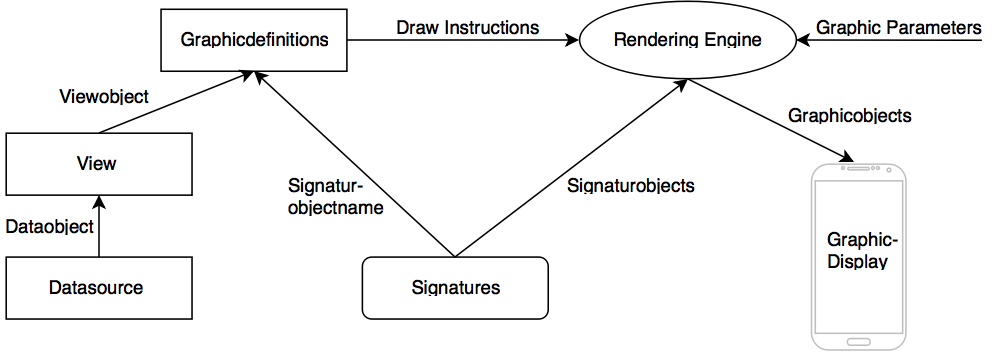
\includegraphics[width=1\textwidth]{images/graphic_definition.png}
  \caption{General graphic definition}
\end{figure}

A layer definition looks like this:
\begin{yamlcode}
- id: landuse
Datasource:
    extent: -20037508.34,-20037508.34,20037508.34,20037508.34
    host: db
    port: 5432
    user: osm
    password: osm
    dbname: osm
    key_field: osm_id
    table: |-
        (
            SELECT osm_id, class, type, geometry
            FROM osm_landusages
            WHERE geometry && !bbox!
            AND z(!scale_denominator!) > 5
        
        ) as data
    type: postgis
fields:
    osm_id: Number
    class: String
    type: String
properties:
    "buffer-size": 4
\end{yamlcode}
The layer definition consist of the id (layername), datasource, fields and the properties. The datasource in this case defines how the postgis database can be accessed and which sql query needs to be executed. But the datasource could also be a geojson, shapefile, sqlite database, geotiff, kml, gpx or csv file.

\subsubsection{Buffers}\label{buffers}
The buffer value on a layer defines how many pixels around each tile will be included. It is necessary to ensure correct rendering across tile boundaries. This value is individual for each layer and depends on the type of data. Buffers for layers containing labels should have a large buffer size such as 128 pixels, whereas a layer like landuse does only need a buffers size of 4 pixels. In general, the buffer size should be set to the minimum to keep the size of the vector tiles as low as possible.\cite{89_mapbox.com_2015}

\begin{figure}[H]
  \centering
  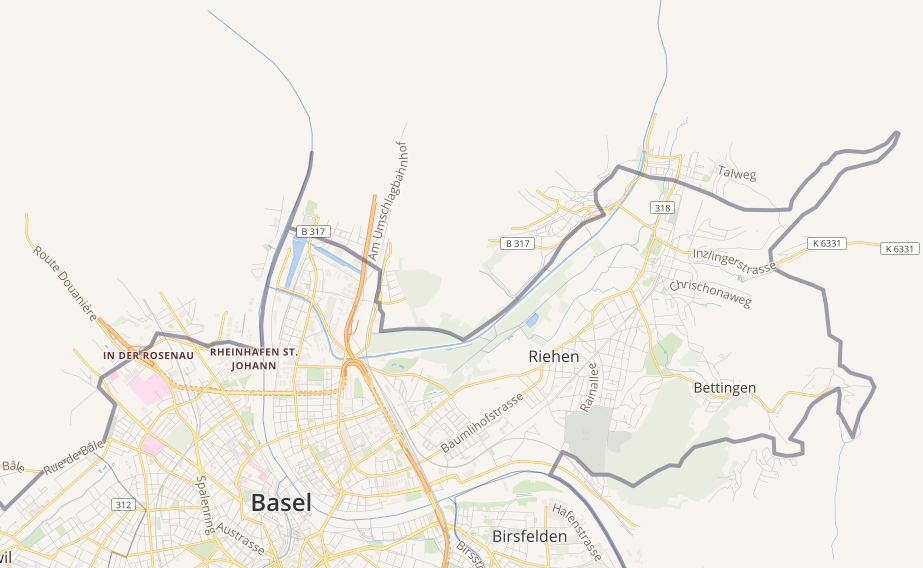
\includegraphics[width=1\textwidth]{images/buffer.png}
  \caption{Example for buffer values}
\end{figure}

The figure above is a good example to see the result of the buffer value. Apart from the rivers there is no other data, therefore the rivers must have a larger buffer value than the other layers.

\subsubsection{Overzooming}\label{overzooming}
The min- and maxzoom values define on which zoom levels there is data. This does not mean that it is not possible to zoom deeper in that the maxzoom value.
Overzooming defines to term of displaying data at higher zoom levels.\cite{90_mapbox.com_2015}
This allows us to show data on higher zoom levels, without generating vector tiles for these zoom levels.
Mapbox has defined a rule of thumb for vector tiles. Vector tiles are useful for about 4-6 levels of overzooming. If I have a vector tile on zoom level 10, it can be stretched out up to zoom level 14 or 16.  

\subsubsection{Layer Ordering}\label{layer_ordering}
The order in which the layer are defined in the data style is equal to the order they are stored in the vector tiles.
The layer at the top of the layer definition will be drawn first next the second layer and so on. So the layer at the bottom is drawn on top of all the other layers.


\section{Zoom Level Reference}\label{zoomlevel_reference}
The zoom level reference helps to see which feature class is included on which zoom level. The zoom levels are ordered by how they get drawn. The feature class landuse is at the bottom and housenum\_label is on top of all the others. 

% Please add the following required packages to your document preamble:
% \usepackage{graphicx}
\begin{table}[H]
\centering
\resizebox{\textwidth}{!}{%
\begin{tabular}{l|ccccccccccccccc}
 & \multicolumn{1}{l}{z0} & \multicolumn{1}{l}{z1} & \multicolumn{1}{l}{z2} & \multicolumn{1}{l}{z3} & \multicolumn{1}{l}{z4} & \multicolumn{1}{l}{z5} & \multicolumn{1}{l}{z6} & \multicolumn{1}{l}{z7} & \multicolumn{1}{l}{z8} & \multicolumn{1}{l}{z9} & \multicolumn{1}{l}{z10} & \multicolumn{1}{l}{z11} & \multicolumn{1}{l}{z12} & \multicolumn{1}{l}{z13} & \multicolumn{1}{l}{z14} \\ \hline
landuse &  &  &  &  &  & x & x & x & x & x & x & x & x & x & x \\
waterway &  &  &  &  &  &  &  &  & x & x & x & x & x & x & x \\
water & x & x & x & x & x & x & x & x & x & x & x & x & x & x & x \\
aeroway &  &  &  &  &  &  &  &  &  &  &  &  & x & x & x \\
barrier\_line &  &  &  &  &  &  &  &  &  &  &  &  &  &  & x \\
building &  &  &  &  &  &  &  &  &  &  &  &  &  & x & x \\
landuse\_overlay &  &  &  &  &  &  &  & x & x & x & x & x & x & x & x \\
tunnel &  &  &  &  &  &  &  &  &  &  &  & x & x & x & x \\
road &  &  &  &  &  & x & x & x & x & x & x & x & x & x & x \\
bridge &  &  &  &  &  &  &  &  &  &  &  &  & x & x & x \\
admin & x & x & x & x & x & x & x & x & x & x & x & x & x & x & x \\
country\_label &  & x & x & x & x & x & x & x & x & x & x & x & x & x & x \\
marine\_label &  & x & x & x & x & x & x & x & x & x & x & x & x & x & x \\
state\_label &  &  &  &  & x & x & x & x & x & x & x & x & x & x & x \\
place\_label &  &  &  &  & x & x & x & x & x & x & x & x & x & x & x \\
water\_label &  &  &  &  &  &  &  &  &  &  & x & x & x & x & x \\
poi\_label &  &  &  &  &  &  &  &  &  &  &  &  &  &  & x \\
road\_label &  &  &  &  &  &  &  &  & x & x & x & x & x & x & x \\
waterway\_label &  &  &  &  &  &  &  &  & x & x & x & x & x & x & x \\
housenum\_label &  &  &  &  &  &  &  &  &  &  &  &  &  &  & x
\end{tabular}
}
\caption{Feature classes on different zoom levels}
\label{my-label}
\end{table}

\section{Reverse Engineering Process}\label{reverse_engineering_process}
One of the main requirements of this project was to make our vector tiles compatible with the Mapbox Streets vector tiles\cite{22_mapbox.com_2015}.
\\
This requirement has not been defined since the beginning, it evolved during the construction of our first prototype.
Therefore a lot of time has been spent making our vector tiles as similar as possible to the ones of Mapbox.
\\
The sections below describe the tools and methods that were used to achieve the goal of Mapbox Streets compatibility.

\subsection{Vector Tile Format}\label{vector_tile_format}
To better understand what the vector tile compare tool does, a high level introduction to the vector tiles format will be given below.
\\\\
A vector tile can consist of one or more named layers and containing one or more features. A feature consist of attributes and a geometry (point, linestring or polygon). Attributes are represented as a dictionary of key, value pairs. 
\\\\
Below you can find an example vector tile, which has two layers water and admin. The water layer has the attribute key "osm\_id" and value 0. If you would compare this example with the specification\cite{4_github_2015}, one could think this is not a specification conform vector tile. The example below is a compressed vector tile. More information on what compression methods are applied can be found in the specification.

Mapbox Streets v6 vector tile(0/0/0):
\begin{jsoncode}
{ 
  "layers": {
    "water": {
      "version": 1,
      "name": "water",
      "extent": 4096,
      "length": 18,
      "_pbf": {
        "buf": [26,143,32,10,5,119,97,1],
        "pos": 51410,
        "length": 51410
      },
      "_keys": ["osm_id"],
      "_values": [0],
      "_features": [11,3474,3499,3530,3561,3584] 
    },
    "admin": {
      "version": 1,
      "name": "admin",
      "extent": 4096,
      "length": 1447,
      "_pbf": {
        "buf": [26,143,32,10,5,1],
        "pos":51410,
        "length":51410
       },
      "_keys": ["admin_level","disputed","iso_3166_1","maritime"],
      "_values": [2,0,"FR",1],
      "_features": [4126,4152,4377,4403,4429,4455,4481,4507,4533]
    }
  } 
}
\end{jsoncode}

\section{Quality Assurance Tools}\label{tools}
During the prototyping phase it was realized, that tools need to be built to help the contributors track the progress of Mapbox Streets compatibility.

\subsection{Vector Tile Compare}\label{vector_tile_compare}
The Vector Tile Compare tool analyzes vector tiles and outputs interesting information like layers and attributes. 
The output was generated for the same vector tiles of Mapbox Streets and the resulting vector tiles from osm2vectortiles (Open Streets).
The results where then uploaded  to a Github repository and the branch compare feature was used to compare them. 

\begin{figure}[H]
  \centering
  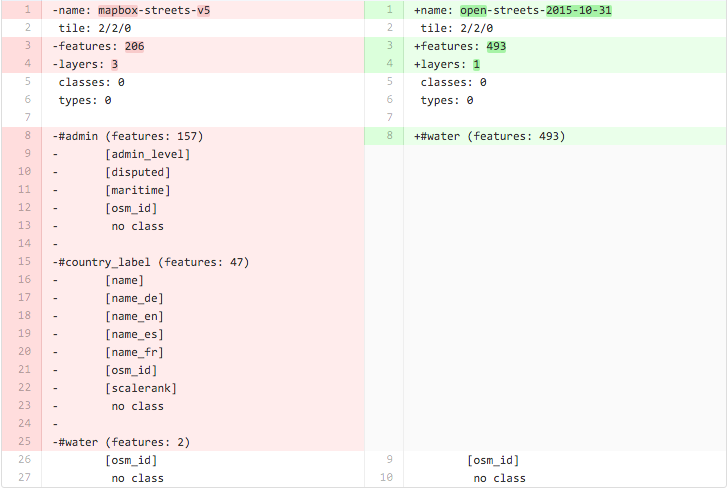
\includegraphics[width=1\textwidth]{images/vector_tile_compare.png}
  \caption{Compare of Mapbox Streets v6 and Open Streets on 31.10.2015}
\end{figure}

This gave us a good indicator of which layers are shown on which zoom level and what attributes are contained in a layer.

\subsection{Visual Compare}\label{visual_compare}
The vector tile comparison was good to ensure that exactly the same data is present on the same zoom level as Mapbox Streets.
But when the contributors started to visually compare the map with the map of Mapbox Streets, big differences appeared.
The decision was made to build a compare tool that works visually to cover up bugs like these.

\begin{figure}[H]
\centering
  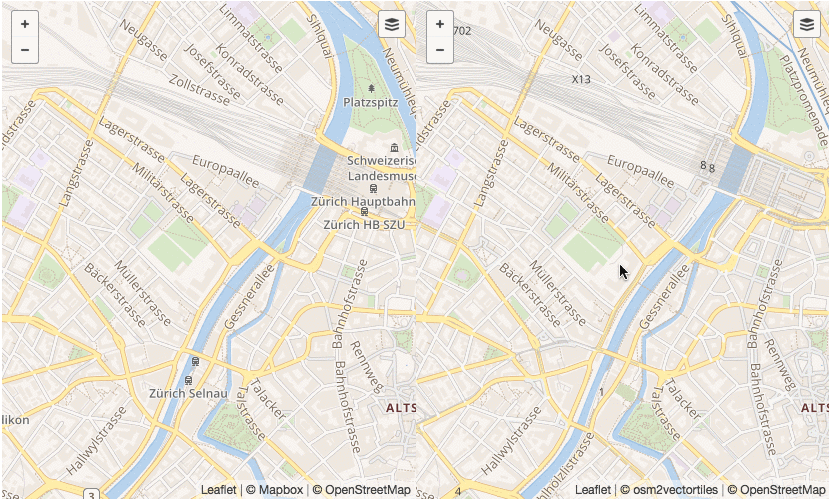
\includegraphics[width=1\textwidth]{images/visual_compare.png}
  \caption{Visual Compare of Mapbox Streets and Open Streets}
\end{figure}

The figure above shows a screenshot of the Visual Compare tool. On the left side is Mapbox Streets and on the right side our Open Streets map. They both use the same visual style (OSM Bright 2\cite{92_github_2015}). When you zoom in on the right side of the map, it automatically zooms in on the left side. This tool was very helpful to find all the differences.

\section{Improvement Process}

This section describes what we did, when we found a visual difference. When we identified a visual difference with the Vector Compare or Visual Compare tool, we first checked if the missing data is included in our import mapping. If this was not the case, we used the TagFinder tool\cite{93_wiki.openstreetmap.org_2015} to find the right OSM key, value pair of the missing item. Next we included the key, value pair into our import mapping and re-imported the OSM data. To see the item on the map, the SQL query in the data style needs to be altered to fetch the added item. Now the missing item should appear on the map. During this process we used mostly Mapbox Studio Classic\cite{mapbox_studio_classic} as the map can be rendered on the fly after the query has been altered.

\section{Limitations}\label{project_limitations}

\paragraph{Tileserver} The tessera based tileserver does not support more than 50 concurrent users and is not meant for production use without a caching reverse proxy in front.

\paragraph{Rendering Workflow} The rendering process is scalable by deploying multiple databases and vector rendering processes on very powerful hosts. For adequate rendering performance at least 16GB (or better 50GB) of memory is required to provide fast database access.
Supporting an additional zoom level 15 would require a significant additional effort in computing capacity for rendering the additional tiles.

\paragraph{Updatable Vector tiles} The vector tiles are based of an OSM planet file at a specific point in time. It is essentially a snapshot of the OSM data. Therefore the Swiss OSM community requested updatable vector tiles based on the diff files.

\paragraph{Base Map} The resulting vector tiles allow creating an alternative base map, which is customizable. The vector tiles are not meant to be queried and do not support custom overlays. Additional map features need to be implemented with the help of other libraries.

\paragraph{OSM Data} The vector tiles contain only a subset of all OSM data. The standard OSM basemap could not easily be replaced with our vector tiles as data source because of this limitation.